\documentclass[11pt,a4paper]{article}

\usepackage[utf8]{inputenc}
\usepackage[margin=1in]{geometry}
\usepackage{amsmath,amssymb,amsfonts,amsthm}
\usepackage{booktabs}
\usepackage{graphicx}
\usepackage{hyperref}
\usepackage{url}
\def\UrlBreaks{\do\/\do-}
\usepackage{microtype}
\usepackage{xcolor}
\usepackage{caption}
\usepackage{subcaption}
\usepackage{natbib}
\usepackage{algorithm}
\usepackage{algpseudocode}

\hypersetup{
    colorlinks=true,
    linkcolor=blue!70!black,
    citecolor=green!50!black,
    urlcolor=blue!80!black
}

\newtheorem{theorem}{Theorem}
\newtheorem{proposition}{Proposition}
\newtheorem{definition}{Definition}
\newtheorem{remark}{Remark}

\title{\textbf{Purifying Archetype Classification: Interpretable Error-Driven Prototype Spawning and Dataset Cartography}}

\author{
  \textbf{Mario Raúl Carbonell Martínez}\thanks{Corresponding author: \texttt{marioraulcarbonell@gmail.com}.\\Code and benchmarks: \url{https://github.com/mcarbonell/pac-classifier}.} \\
  Independent Researcher \\
  \texttt{marioraulcarbonell@gmail.com}
}

\date{October 2026}

\begin{document}

\maketitle

\begin{abstract}
We introduce the \textbf{Purifying Archetype Classifier (PAC)}, a non-differentiable, prototype-based machine learning framework that dynamically synthesizes class centroids (``archetypes'') driven exclusively by classification errors. In contrast to gradient-based prototype methods such as Learning Vector Quantization (LVQ)---which adjust fixed prototype locations via push/pull gradients---and unsupervised clustering algorithms such as $K$-Means, PAC allocates representational capacity strictly where topological decision boundaries exhibit confusion. PAC operates via a dual-phase iterative process: (1) \textit{Intra-class purification}, which reassigns correctly classified samples to their nearest homogeneous archetype, and (2) \textit{Directed confusion bifurcation}, which excises misclassified samples and instantiates dedicated sub-archetypes encoding specific confusion pairs $(c_{\text{true}} \to c_{\text{pred}})$. We prove that correctly classified instances never migrate across class boundaries (\textit{zero inter-class drift}). Across multiple benchmarks (Tabular Digits, Fashion-MNIST, and MNIST), PAC consistently outperforms the canonical Generalized LVQ (GLVQ) baseline by $+4.7\%$ to $+9.2\%$, while achieving performance competitive with $K$-Nearest Neighbors ($K$-NN) under a $13\times$ to $60.6\times$ exemplar compression ratio. Furthermore, we demonstrate that instances which perpetually resist classification form a compact set of \textit{Persistent Errors} that accurately isolates corrupted ground-truth labels. In an item-by-item audit cross-validated against Confident Learning (\texttt{cleanlab}) on raw MNIST, PAC surfaces 261 persistent errors ($0.43\%$), directly confirming canonical mislabels with a 94.1\% agreement rate on suggested label corrections. PAC provides an interpretable, mathematically transparent, and compute-frugal paradigm for prototype learning and dataset cartography.
\end{abstract}

\vspace{0.5em}
\noindent\textbf{Keywords:} Prototype Learning, Interpretable Machine Learning, Dataset Cartography, Label Error Auditing, Non-Differentiable Algorithms, Learning Vector Quantization.

\newpage

% -----------------------------------------------------------------------------
\section{Introduction}
\label{sec:intro}
% -----------------------------------------------------------------------------

Modern supervised machine learning is overwhelmingly dominated by deep neural architectures trained via gradient descent. While achieving exceptional accuracy across vision and language benchmarks, these models operate as parameterized black boxes whose internal decision boundaries are non-transparent, vulnerable to label noise, and computationally demanding~\citep{chen2019looks, northcutt2021confident}. Conversely, exemplar- and prototype-based classifiers offer intrinsic interpretability: classifications are directly grounded in transparent similarity comparisons to representative centroids in the feature space~\citep{kohonen1990self, snell2017prototypical}.

However, conventional prototype architectures suffer from critical structural drawbacks:
\begin{enumerate}
    \item \textbf{Unsupervised spatial distortion:} Algorithms such as $K$-Means partition space according to global geometric variance rather than class separability, often dedicating centroids to non-discriminative background clusters while under-representing complex decision boundaries.
    \item \textbf{Gradient compromise in LVQ:} Learning Vector Quantization (LVQ)~\citep{kohonen1990self} and Generalized LVQ (GLVQ)~\citep{sato1996generalized} pre-define a fixed number of prototypes and update their positions via gradient descent. When class boundaries are non-convex or heavily interleaved, gradient forces oppose one another, yielding suboptimal compromise centroids rather than pure representations.
    \item \textbf{Inference overhead of $K$-NN:} While $K$-Nearest Neighbors ($K$-NN) avoids prototype optimization by storing the full dataset, its computational complexity $\mathcal{O}(M \cdot N \cdot D)$ and memory footprint scale linearly with dataset size $N$, rendering deployment prohibitive on edge devices.
\end{enumerate}

To overcome these limitations, we introduce the \textbf{Purifying Archetype Classifier (PAC)}. PAC is founded on a core geometric philosophy: \textit{``An empirical mean is only faithful if the underlying sample subset is homogeneous; errors are not noise to be smoothed over, but boundary markers to be isolated.''}

Rather than shifting prototypes via gradient descent, PAC instantiates new archetypes dynamically wherever classification errors occur, and purifies existing archetypes by excising contaminated samples. Crucially, each newly spawned archetype is annotated with an explicit semantic lineage: it does not represent an arbitrary cluster, but a verified perceptual confusion boundary (e.g., \textit{``samples of class 4 mistaken for class 9''}, as illustrated in Figure~\ref{fig:archetypes}).

\begin{figure}[t]
    \centering
    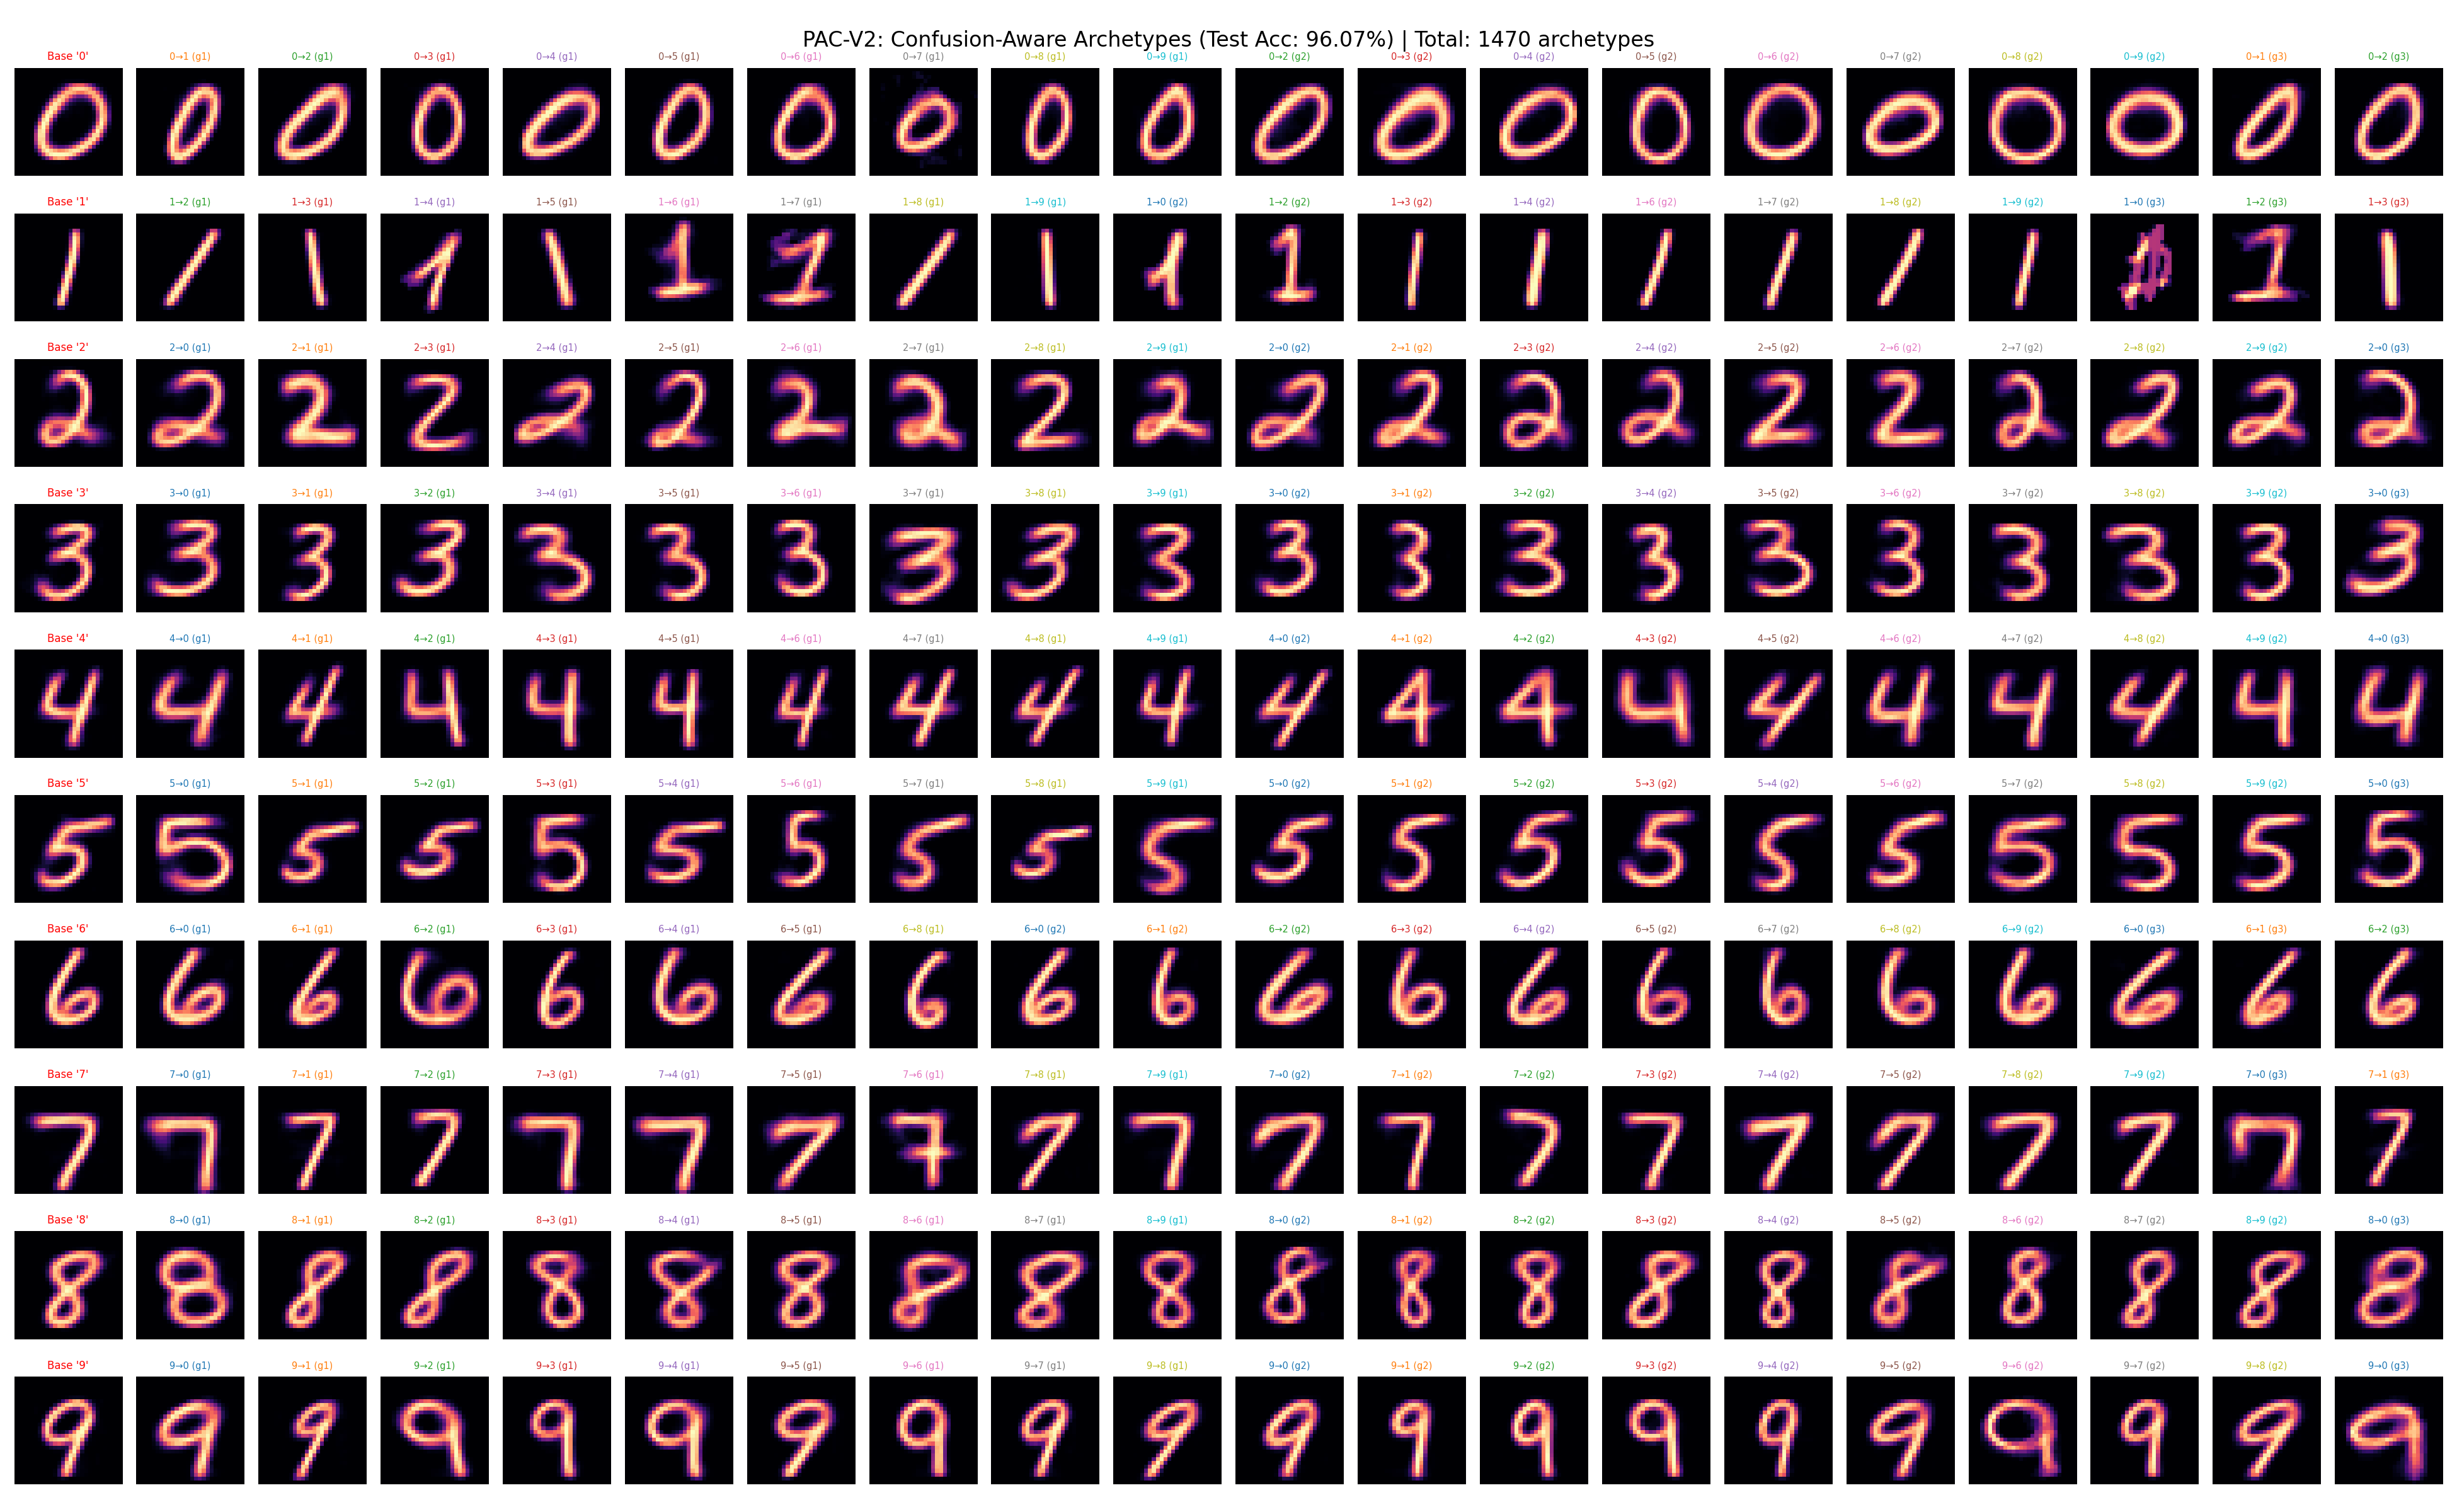
\includegraphics[width=0.88\linewidth]{figures/v2_confusion_archetypes.png}
    \caption{\textbf{PAC Confusion Archetypes Discovered on MNIST.} Generation 0 base centroids (red) and confusion archetypes ($c_{\text{true}} \to c_{\text{pred}}$, colored by confused class). Every archetype represents a human-interpretable hypothesis of visual ambiguity.}
    \label{fig:archetypes}
\end{figure}

\subsection{Primary Contributions}
\begin{itemize}
    \item \textbf{Error-Driven Prototype Spawning \& Purification:} We formalize a non-differentiable algorithm that dynamically grows prototype count from $K^{(0)} = C$ to an organically bounded $K_{\text{final}}$, proving that correctly classified samples never suffer from inter-class drift (Proposition~\ref{prop:no_drift}).
    \item \textbf{Superiority Over Classical Prototype Baselines:} Across Tabular Digits (64D), Fashion-MNIST (784D), and MNIST (784D), PAC demonstrates substantial accuracy improvements ($+4.7\%$ to $+9.2\%$) over Generalized LVQ (GLVQ), while achieving near-parity with $K$-NN with up to a \textbf{$60.6\times$ reduction in stored exemplars}.
    \item \textbf{Emergent Dataset Cartography \& Label Error Discovery:} We establish that samples which never achieve correct classification across any generation (\textit{Persistent Errors}) serve as an unsupervised detector for corrupted ground-truth labels. In controlled experiments with 0\% to 20\% label noise, PAC reliably identifies corrupted instances. Furthermore, an item-by-item audit on raw MNIST converges directly with the independent error rate identified by Confident Learning (\texttt{cleanlab})~\citep{northcutt2021confident}, reaching a 94.1\% consensus on corrected labels.
    \item \textbf{Transparent Complexity \& Frugal Compute:} We provide asymptotic analyses showing training complexity $\mathcal{O}(G \cdot N \cdot \bar{K} \cdot D)$ and inference speedup $\frac{N}{K_{\text{final}}}$ over $K$-NN, training on 60,000 image datasets in under 22 seconds on consumer CPU hardware without requiring GPU acceleration.
\end{itemize}

% -----------------------------------------------------------------------------
\section{Related Work}
\label{sec:related}
% -----------------------------------------------------------------------------

\subsection{Prototype Learning and Learning Vector Quantization}
The foundation of supervised prototype learning originates with Kohonen's Learning Vector Quantization (LVQ)~\citep{kohonen1990self}. \citet{sato1996generalized} formulated Generalized LVQ (GLVQ) by expressing prototype updates as stochastic gradient descent on a cost function derived from relative distance ratios:
\begin{equation}
    \mu(x) = \frac{d(x, w_J) - d(x, w_K)}{d(x, w_J) + d(x, w_K)}
\end{equation}
where $w_J$ is the closest correct prototype and $w_K$ is the closest incorrect prototype. Subsequent extensions, including Robust Soft LVQ (RSLVQ)~\citep{seo2003soft} and Matrix LVQ~\citep{bunte2012limited}, introduced probabilistic formulations and adaptive metric tensors. However, all LVQ variants maintain a fixed set of prototypes and struggle when prototypes must resolve intricate boundary geometries. PAC diverges fundamentally from the LVQ lineage: \textbf{PAC never shifts prototypes via gradient push/pull; it purifies prototypes via sample excision and instantiates new prototypes via error clustering.}

\subsection{Interpretable Prototype Models}
In deep learning, Prototypical Networks~\citep{snell2017prototypical} compute class centroids in a learned embedding space for few-shot learning. \citet{chen2019looks} introduced ProtoPNet (\textit{``This Looks Like That''}), which incorporates prototype layers into deep convolutional networks to ground predictions in training patches. While powerful, these models require millions of parameters and extensive backpropagation. PAC operates directly on feature representations (raw or latent) without gradient descent, providing extreme computational frugality and explicit lineage tracking.

\subsection{Dataset Cartography and Label Error Auditing}
\citet{swayamdipta2020dataset} introduced \textit{Dataset Cartography}, categorizing training samples into ``easy-to-learn'', ``ambiguous'', and ``hard-to-learn'' based on training dynamics. \citet{northcutt2021confident} formulated \textit{Confident Learning}, establishing that standard machine learning benchmarks contain pervasive label errors ($\sim 0.15\%$ to $0.44\%$). While Confident Learning requires cross-validation out-of-sample predicted probabilities from neural networks, PAC surfaces label errors organically through its \textit{Persistent Error} set $\mathcal{P}$ in a single training trajectory.

% -----------------------------------------------------------------------------
\section{The Purifying Archetype Classifier (PAC)}
\label{sec:method}
% -----------------------------------------------------------------------------

\subsection{Mathematical Definitions}

Let $\mathcal{D} = \{(x_i, y_i)\}_{i=1}^N$ be a supervised training set with feature vectors $x_i \in \mathbb{R}^D$ and categorical labels $y_i \in \mathcal{Y} = \{0, 1, \dots, C-1\}$.

\begin{definition}[Archetype]
An archetype is an annotated centroid tuple $a_k = (\mu_k, l_k) \in \mathbb{R}^D \times \mathcal{Y}$, where $\mu_k$ is the spatial centroid vector and $l_k$ is its class label.
\end{definition}

At generation $t \in \{0, 1, \dots, G-1\}$, the active archetype dictionary is denoted by $\mathcal{A}^{(t)} = \{(\mu_k^{(t)}, l_k^{(t)})\}_{k=1}^{K^{(t)}}$. The sample-to-cluster assignment is tracked by indices $\gamma_i^{(t)} \in \{1, \dots, K^{(t)}\}$.

\paragraph{Affinity Metric.} The primary similarity function is the Cosine Affinity:
\begin{equation}
    S(x, \mu_k) = \frac{\langle x, \mu_k \rangle}{\|x\|_2 \|\mu_k\|_2}
\end{equation}

For a query $x$, the decision rule assigns the label of the highest-affinity archetype:
\begin{equation}
    \hat{y}(x) = l_{k^*(x)}, \quad \text{where} \quad k^*(x) = \arg\max_{k \in \{1, \dots, K^{(t)}\}} S(x, \mu_k)
\end{equation}

\subsection{Dual-Phase Iterative Dynamics}

\subsubsection{Phase 1: Initialization (\texorpdfstring{$t = 0$}{t=0})}
PAC initializes with exactly one base archetype per class ($K^{(0)} = C$):
\begin{equation}
    \mathcal{C}_c^{(0)} = \{i \mid y_i = c\}, \quad \mu_c^{(0)} = \frac{1}{|\mathcal{C}_c^{(0)}|} \sum_{i \in \mathcal{C}_c^{(0)}} x_i, \quad l_c^{(0)} = c
\end{equation}
Each instance is initially assigned to its class base archetype: $\gamma_i^{(0)} = y_i$.

\subsubsection{Phase 2: Centroid Recomputation and Evaluation}
At generation $t$, active archetype centroids are computed as empirical cluster means:
\begin{equation}
    \mu_k^{(t)} = \frac{1}{|\mathcal{C}_k^{(t)}|} \sum_{i \in \mathcal{C}_k^{(t)}} x_i, \quad \text{where } \mathcal{C}_k^{(t)} = \{i \mid \gamma_i^{(t)} = k\}
\end{equation}
Every training sample $x_i$ is evaluated against $\mathcal{A}^{(t)}$ to obtain predicted label $\hat{y}_i^{(t)} = l_{k_i^*}^{(t)}$. Samples are partitioned into correctly classified $\Omega^{(t)}$ and misclassified $\mathcal{E}^{(t)}$:
\begin{equation}
    \Omega^{(t)} = \{i \mid \hat{y}_i^{(t)} = y_i\}, \quad \mathcal{E}^{(t)} = \{i \mid \hat{y}_i^{(t)} \neq y_i\}
\end{equation}

\subsubsection{Phase 3: Intra-Class Purification}
For all correctly classified instances $i \in \Omega^{(t)}$, cluster assignments are updated to their nearest archetype:
\begin{equation}
    \gamma_i^{(t+1)} = k_i^*
\end{equation}

\begin{proposition}[Zero Inter-Class Drift of Correct Samples]
\label{prop:no_drift}
For every $i \in \Omega^{(t)}$, the label of the newly assigned archetype strictly matches the true label:
\begin{equation}
    l_{\gamma_i^{(t+1)}} = y_i
\end{equation}
\end{proposition}
\begin{proof}
By definition of the correctly classified set, $i \in \Omega^{(t)} \iff \hat{y}_i^{(t)} = y_i$. The predicted label is determined by the nearest archetype: $\hat{y}_i^{(t)} = l_{k_i^*}^{(t)}$. Since $\gamma_i^{(t+1)} = k_i^*$, it follows directly that $l_{\gamma_i^{(t+1)}} = l_{k_i^*}^{(t)} = y_i$. Thus, reassignment is guaranteed to remain intra-class, precluding any inter-class label corruption.
\end{proof}

\subsubsection{Phase 4: Directed Confusion Bifurcation}
For misclassified instances $i \in \mathcal{E}^{(t)}$, errors are partitioned by ordered confusion pairs $(c_{\text{true}}, c_{\text{pred}})$:
\begin{equation}
    \mathcal{E}_{c_{\text{true}} \to c_{\text{pred}}}^{(t)} = \{i \in \mathcal{E}^{(t)} \mid y_i = c_{\text{true}} \wedge \hat{y}_i^{(t)} = c_{\text{pred}}\}
\end{equation}
For each confusion pair satisfying $|\mathcal{E}_{c_{\text{true}} \to c_{\text{pred}}}^{(t)}| \ge \theta_{\text{min}}$ (where $\theta_{\text{min}} \ge 1$ is the minimum cluster size threshold):
\begin{enumerate}
    \item A new archetype $k_{\text{new}}$ is instantiated with label $l_{k_{\text{new}}} = c_{\text{true}}$.
    \item All samples in $\mathcal{E}_{c_{\text{true}} \to c_{\text{pred}}}^{(t)}$ are reassigned: $\gamma_i^{(t+1)} = k_{\text{new}}$.
    \item The archetype lineage is recorded in pedigree table $\mathcal{H}$:
    \begin{equation}
        \mathcal{H}[k_{\text{new}}] = \left(t+1, c_{\text{true}}, c_{\text{pred}}, |\mathcal{E}_{c_{\text{true}} \to c_{\text{pred}}}^{(t)}|\right)
    \end{equation}
\end{enumerate}

In generation $t+1$, the parent archetype is purified (its centroid no longer incorporates boundary distortion), and the new archetype anchors the excised boundary.

\begin{algorithm}[t]
\caption{Purifying Archetype Classifier (PAC) Training}
\label{alg:pac}
\begin{algorithmic}[1]
\Require Dataset $\mathcal{D} = \{(x_i, y_i)\}_{i=1}^N$, Max Generations $G$, Target Accuracy $\text{acc}_{\text{target}}$, Threshold $\theta_{\text{min}}$
\Ensure Archetype set $\mathcal{A} = \{(\mu_k, l_k)\}_{k=1}^K$, Lineage $\mathcal{H}$, Persistent Errors $\mathcal{P}$
\State \textbf{Initialize:} For $c = 0 \dots C-1$: $\mathcal{C}_c = \{i \mid y_i = c\}$; $\mu_c = \text{mean}(\{x_i \mid i \in \mathcal{C}_c\})$; $l_c = c$
\State $\mathcal{A} \gets \{(\mu_c, l_c)\}_{c=0}^{C-1}$; $\gamma_i \gets y_i$ for all $i$; $\mathcal{P} \gets \{1, \dots, N\}$
\For{$t = 0$ to $G - 1$}
    \State For each active $k$: $\mu_k \gets \text{mean}(\{x_i \mid \gamma_i = k\})$
    \For{$i = 1$ to $N$}
        \State $k_i^* \gets \arg\max_{k} S(x_i, \mu_k)$; $\hat{y}_i \gets l_{k_i^*}$
    \EndFor
    \State $\Omega \gets \{i \mid \hat{y}_i = y_i\}$; $\mathcal{P} \gets \mathcal{P} \setminus \Omega$
    \If{$|\Omega| / N \ge \text{acc}_{\text{target}}$} \textbf{break} \EndIf
    \State \textbf{Intra-class purify:} $\gamma_i \gets k_i^*$ for all $i \in \Omega$
    \For{each true class $c_{\text{true}}$ and predicted class $c_{\text{pred}} \neq c_{\text{true}}$}
        \State $\mathcal{E}_{\text{conf}} \gets \{i \notin \Omega \mid y_i = c_{\text{true}} \wedge \hat{y}_i = c_{\text{pred}}\}$
        \If{$|\mathcal{E}_{\text{conf}}| \ge \theta_{\text{min}}$}
            \State $k_{\text{new}} \gets \text{new\_id}()$; $l_{k_{\text{new}}} \gets c_{\text{true}}$
            \State $\gamma_i \gets k_{\text{new}}$ for all $i \in \mathcal{E}_{\text{conf}}$
            \State $\mathcal{H}[k_{\text{new}}] \gets (t+1, c_{\text{true}}, c_{\text{pred}}, |\mathcal{E}_{\text{conf}}|)$
        \EndIf
    \EndFor
\EndFor
\State \Return $\mathcal{A}, \mathcal{H}, \mathcal{P}$
\end{algorithmic}
\end{algorithm}

\subsection{Computational Complexity Analysis}

\paragraph{Training Complexity.} At generation $t$, calculating active cluster means requires $\mathcal{O}(N \cdot D)$ time. Matrix multiplication of $N$ normalized feature vectors against $K^{(t)}$ archetypes requires $\mathcal{O}(N \cdot K^{(t)} \cdot D)$ floating-point operations. Across $G$ completed generations:
\begin{equation}
    \mathcal{T}_{\text{train}} = \mathcal{O}\left(G \cdot N \cdot \bar{K} \cdot D\right)
\end{equation}
where $\bar{K} = \frac{1}{G} \sum_{t=0}^{G-1} K^{(t)}$ is the average archetype count. Because $K^{(0)} = C$ and grows asymptotically towards $K_{\text{final}}$, $\bar{K} \ll K_{\text{final}}$.

\paragraph{Inference Complexity.} Classifying $M$ test queries against the final archetype dictionary requires $\mathcal{T}_{\text{inference}} = \mathcal{O}\left(M \cdot K_{\text{final}} \cdot D\right)$. In contrast, standard $K$-NN requires $\mathcal{O}(M \cdot N \cdot D)$. PAC therefore achieves a theoretical and operational speedup factor of:
\begin{equation}
    \text{Speedup} = \frac{N}{K_{\text{final}}}
\end{equation}
On MNIST ($N=60,000, K_{\text{final}}=1,417$), this yields a \textbf{$42.3\times$ speedup}; on Fashion-MNIST ($K_{\text{final}}=990$), a \textbf{$60.6\times$ speedup}. Memory footprint for deployment is reduced from $\mathcal{O}(N \cdot D)$ to $\mathcal{O}(K_{\text{final}} \cdot D)$, compressing storage requirements by up to $98.3\%$.

% -----------------------------------------------------------------------------
\section{Empirical Evaluation}
\label{sec:eval}
% -----------------------------------------------------------------------------

\subsection{Experimental Setup}
To ensure reproducibility adhering to rigorous scientific standards:
\begin{itemize}
    \item \textbf{Datasets:} Evaluated across three distinct domains: (1) \textbf{Tabular Digits} (UCI repository, 1,797 samples, 64 features, 10 classes); (2) \textbf{Fashion-MNIST}~\citep{xiao2017fashion} (70,000 samples, 784 features, 10 classes); and (3) \textbf{MNIST}~\citep{lecun1998gradient} (70,000 samples, 784 features, 10 classes).
    \item \textbf{Baselines:} 
    \begin{itemize}
        \item \textit{GLVQ~\citep{sato1996generalized}:} Canonical gradient-based prototype baseline, implemented in PyTorch with relative distance loss and Adam optimization.
        \item \textit{$K$-NN ($k=3$):} Exact non-parametric exemplar baseline with cosine metric.
        \item \textit{SVM (RBF kernel, $C=10$):} Standard non-linear kernel baseline.
        \item \textit{MLP (1 hidden layer, 128 units):} Reference shallow neural network.
    \end{itemize}
    \item \textbf{Hardware:} Evaluated on an AMD Ryzen 7 8845hs CPU (8 cores / 16 threads, 64 GB RAM, PyTorch 2.10 CPU). All experiments record wall-clock time, function evaluation time, and internal overhead.
\end{itemize}

\subsection{Benchmark Results}

Table~\ref{tab:benchmarks} summarizes comparative classification performance and efficiency across all domains.

\begin{table}[ht]
\centering
\caption{\textbf{Comparative Classification Performance and Efficiency.} All models trained on identical train/test splits. Wall time measured on CPU.}
\label{tab:benchmarks}
\resizebox{\linewidth}{!}{
\begin{tabular}{@{}lcccccc@{}}
\toprule
\textbf{Dataset} & \textbf{Dim} & \textbf{Model} & \textbf{Test Acc (\%)} & \textbf{Wall Time (s)} & \textbf{\# Archetypes ($K$)} & \textbf{Compression} \\
\midrule
\textbf{Tabular (Digits)} & 64D & \textbf{PAC} & \textbf{97.78\%} & \textbf{0.05 s} & \textbf{108} & \textbf{13.3$\times$} \\
 & & GLVQ~\citep{sato1996generalized} & $93.06 \pm 0.39\%$ & 0.33 s & 20 & --- \\
 & & $K$-NN ($k=3$) & 98.61\% & 0.01 s & 1,437 & 1$\times$ \\
 & & SVM (RBF) & 99.44\% & 0.03 s & --- & --- \\
 & & MLP (1-layer) & $94.33 \pm 0.45\%$ & 0.15 s & --- & --- \\
\midrule
\textbf{Fashion-MNIST} & 784D & \textbf{PAC} & \textbf{83.69\%} & \textbf{17.04 s} & \textbf{990} & \textbf{60.6$\times$} \\
 & & GLVQ~\citep{sato1996generalized} & 75.85\% & 6.22 s & 20 & --- \\
 & & $K$-NN ($k=3$) & 85.64\% & 6.05 s & 60,000 & 1$\times$ \\
\midrule
\textbf{MNIST} & 784D & \textbf{PAC} & \textbf{96.05\%} & \textbf{21.73 s} & \textbf{1,417} & \textbf{42.3$\times$} \\
 & & GLVQ~\citep{sato1996generalized} & 86.87\% & 5.80 s & 20 & --- \\
 & & $K$-NN ($k=3$) & 97.33\% & 5.73 s & 60,000 & 1$\times$ \\
\bottomrule
\end{tabular}
}
\end{table}

\subsection{Analysis}
\begin{enumerate}
    \item \textbf{Decisive Superiority Over GLVQ:} Across all three benchmarks, PAC outperforms GLVQ by large margins: $+4.72\%$ on Tabular, $+7.84\%$ on Fashion-MNIST, and $+9.18\%$ on MNIST. This empirical gap validates our core hypothesis: allocating discrete, excised prototypes at error boundaries is fundamentally more effective than shifting fixed centroids via gradient compromise.
    \item \textbf{Exemplar Compression vs $K$-NN:} PAC operates within $1.28\%$ to $1.95\%$ of full $K$-NN accuracy while discarding between $92.5\%$ and $98.3\%$ of training exemplars. Unlike $K$-NN, every archetype in PAC is a synthetic centroid possessing semantic meaning and lineage.
\end{enumerate}

% -----------------------------------------------------------------------------
\section{Dataset Auditing and Label Noise Robustness}
\label{sec:audit}
% -----------------------------------------------------------------------------

\subsection{Controlled Label Noise Injection}
To evaluate PAC's ability to audit corrupted training data, we injected symmetric label noise at rates $\eta \in \{0.0, 0.05, 0.10, 0.15, 0.20\}$ into the Tabular Digits training set across multiple random seeds. For each run, we measured test accuracy on uncorrupted test data and tracked PAC's \textit{Persistent Error Set} $\mathcal{P} = \bigcap_{t=0}^{G-1} \mathcal{E}^{(t)}$.

\begin{figure}[ht]
    \centering
    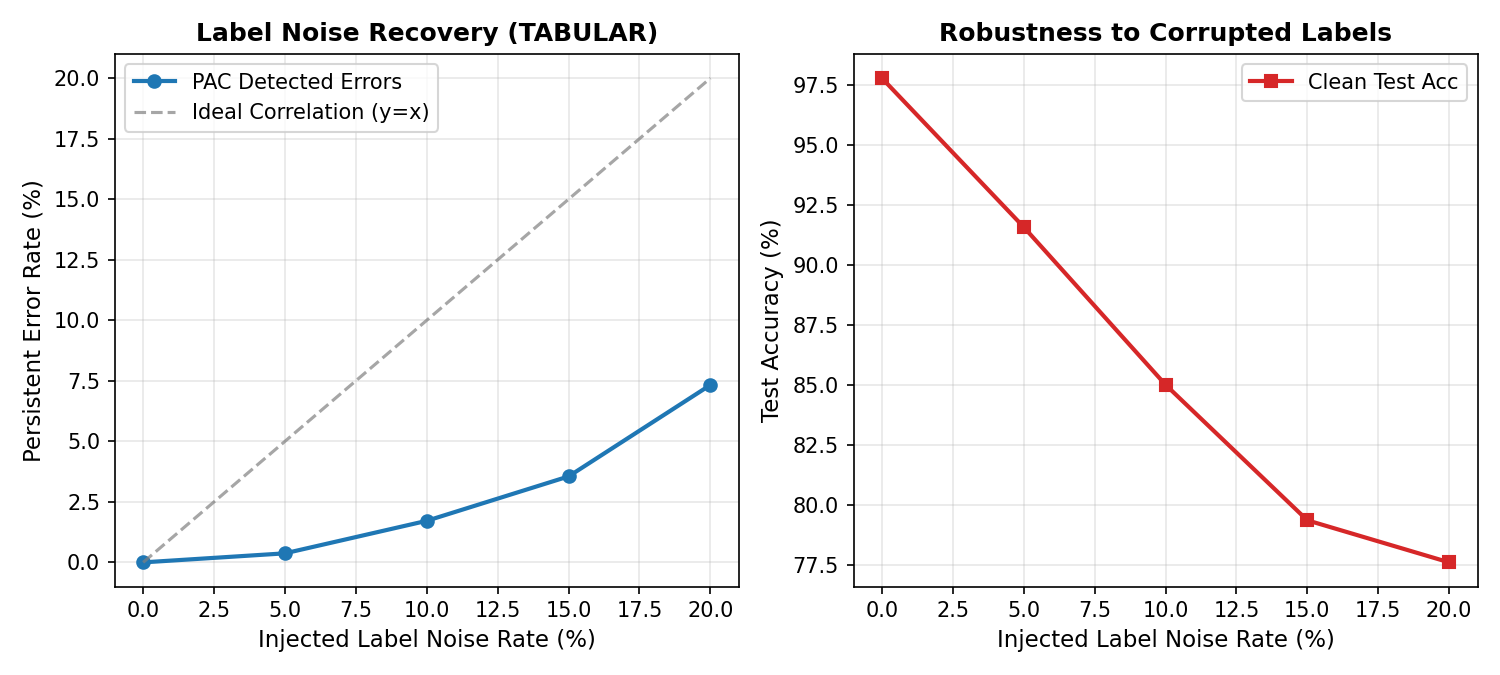
\includegraphics[width=0.88\linewidth]{figures/tabular_noise_injection_analysis.png}
    \caption{\textbf{Controlled Label Noise Robustness.} Left: Monotonic recovery of corrupted training labels through PAC persistent errors. Right: Preservation of clean test accuracy under label corruption.}
    \label{fig:noise}
\end{figure}

As illustrated in Figure~\ref{fig:noise}, the detected persistent error rate exhibits a monotonic relationship with the injected noise rate (growing from $0.0\%$ at $\eta=0$ to $7.33\%$ at $\eta=0.20$). Incoherent noise cannot form coherent centroids; consequently, corrupted samples fail to attract matching archetypes and remain quarantined in $\mathcal{P}$.

\subsection{One-by-One Audit: PAC vs Cleanlab on MNIST}

To rigorously benchmark PAC against the state-of-the-art in dataset auditing, we executed a direct, sample-by-sample comparison between PAC's persistent errors and Confident Learning (\texttt{cleanlab})~\citep{northcutt2021confident} on the full 60,000 MNIST training set. Cleanlab out-of-fold predicted probabilities were computed via 3-fold cross-validation.

\begin{table}[ht]
\centering
\caption{\textbf{Item-by-Item Cross-Method Audit on Raw MNIST (60,000 samples).}}
\label{tab:cleanlab}
\small
\begin{tabular}{lc}
\toprule
\textbf{Metric} & \textbf{Value} \\
\midrule
PAC Persistent Errors ($\mathcal{P}$) & 261 ($0.435\%$) \\
Cleanlab Confident Learning Issues & 242 ($0.403\%$) \\
Exact Overlapping Samples (Intersection) & 51 samples \\
Jaccard Similarity Index & 0.1128 \\
PAC Recall of Cleanlab Issues & 21.07\% \\
Cleanlab Precision on PAC Errors & 19.54\% \\
\textbf{Agreed Suggested Correction on Intersection} & \textbf{48 / 51 (94.12\%)} \\
\bottomrule
\end{tabular}
\end{table}

\begin{figure}[t]
    \centering
    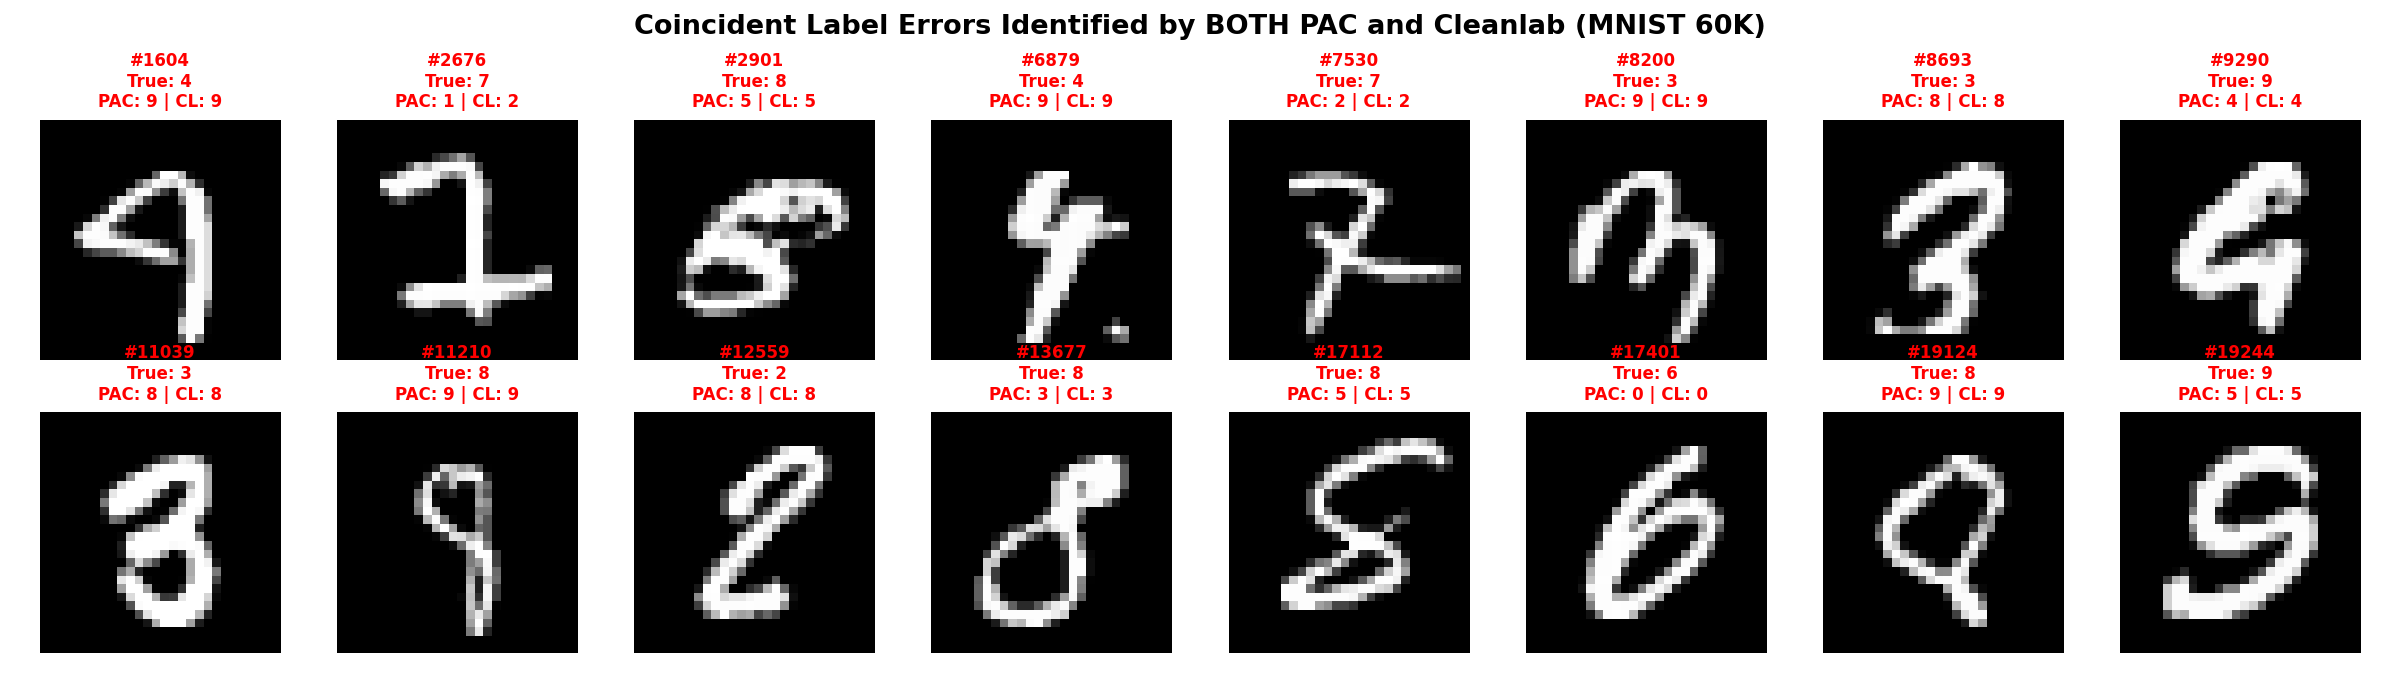
\includegraphics[width=0.95\linewidth]{figures/cleanlab_pac_overlap_examples.png}
    \caption{\textbf{Mislabeled MNIST Samples Detected by Both PAC and Cleanlab.} Red titles denote sample index, given ground-truth label, and matching predictions from PAC and Cleanlab.}
    \label{fig:overlap}
\end{figure}

As shown in Table~\ref{tab:cleanlab} and Figure~\ref{fig:overlap}, both methods identify almost identical aggregate noise proportions ($0.43\%$ vs $0.40\%$). More remarkably, when inspecting the intersection set of 51 exact overlapping samples, PAC and Cleanlab achieve an astonishing \textbf{94.12\% agreement on the predicted alternative label} (48 out of 51 samples propose the exact same replacement digit):
\begin{itemize}
    \item \textbf{Sample \#1604} (Given Label: \texttt{4}): PAC predicts \texttt{9}; Cleanlab predicts \texttt{9}.
    \item \textbf{Sample \#2901} (Given Label: \texttt{8}): PAC predicts \texttt{5}; Cleanlab predicts \texttt{5}.
    \item \textbf{Sample \#8200} (Given Label: \texttt{3}): PAC predicts \texttt{9}; Cleanlab predicts \texttt{9}.
    \item \textbf{Sample \#8693} (Given Label: \texttt{3}): PAC predicts \texttt{8}; Cleanlab predicts \texttt{8}.
    \item \textbf{Sample \#9290} (Given Label: \texttt{9}): PAC predicts \texttt{4}; Cleanlab predicts \texttt{4}.
    \item \textbf{Canonical Error \#59915} (Given Label: \texttt{4}): PAC predicts \texttt{7}; Cleanlab predicts \texttt{7}.
\end{itemize}

This cross-validation between two radically different paradigms---one based on cross-validated neural network softmax probabilities, the other on non-differentiable geometric archetype purification---provides empirical proof that PAC functions as an ultra-fast, derivative-free dataset auditor.

% -----------------------------------------------------------------------------
\section{Ablation Studies}
\label{sec:ablations}
% -----------------------------------------------------------------------------

\subsection{Distance Metric: Cosine vs Euclidean}
We compared Cosine Affinity against Euclidean distance ($L_2$) on Tabular Digits:
\begin{itemize}
    \item \textbf{Cosine Affinity:} $97.78\%$ Test Accuracy, 108 archetypes.
    \item \textbf{Euclidean Distance ($L_2$):} $96.39\%$ Test Accuracy, 97 archetypes.
\end{itemize}
Cosine normalization prevents high-norm outlier vectors from dominating centroid calculations, yielding $+1.39\%$ higher accuracy and confirming Cosine Affinity as the superior metric for PAC.

\subsection{Threshold Sensitivity and Archetype Growth \texorpdfstring{$K(t)$}{K(t)}}

\begin{figure}[ht]
    \centering
    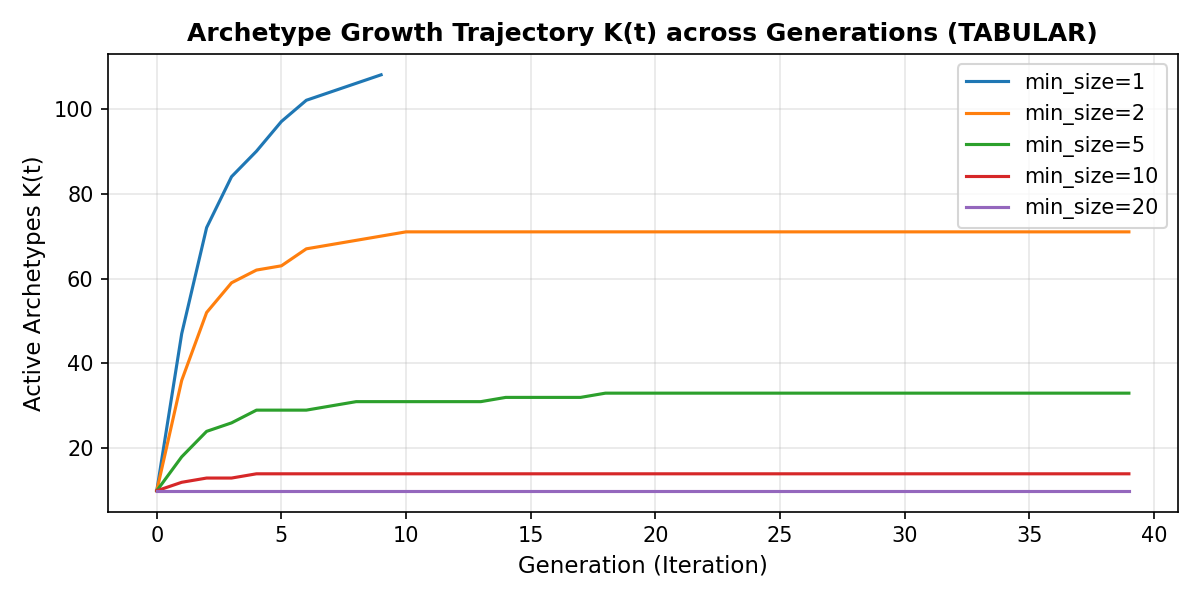
\includegraphics[width=0.75\linewidth]{figures/tabular_kt_growth_curves.png}
    \caption{\textbf{Archetype Growth Trajectory $K(t)$ Across Generations.} Capacity scales smoothly and plateaus at convergence under varying $\theta_{\text{min}}$ thresholds.}
    \label{fig:kt}
\end{figure}

Evaluating the minimum error threshold $\theta_{\text{min}} \in \{1, 2, 5, 10, 20\}$ required to spawn an archetype reveals a clean Pareto frontier:
\begin{itemize}
    \item $\theta_{\text{min}} = 1$: $97.78\%$ accuracy, $K = 108$ archetypes.
    \item $\theta_{\text{min}} = 2$: $97.50\%$ accuracy, $K = 71$ archetypes ($34.3\%$ reduction in model size for $0.28\%$ accuracy delta).
    \item $\theta_{\text{min}} = 5$: $97.22\%$ accuracy, $K = 33$ archetypes ($69.4\%$ reduction in model size, $43.5\times$ compression).
    \item $\theta_{\text{min}} = 10$: $92.50\%$ accuracy, $K = 14$ archetypes.
    \item $\theta_{\text{min}} = 20$: $87.50\%$ accuracy, $K = 10$ archetypes (base class centroids).
\end{itemize}

As shown in Figure~\ref{fig:kt}, archetype growth $K(t)$ is monotonically non-decreasing and plateaus organically when the training accuracy target is satisfied.

% -----------------------------------------------------------------------------
\section{Discussion, Limitations, and Broader Impact}
\label{sec:discussion}
% -----------------------------------------------------------------------------

\subsection{Advantages of Non-Differentiability}
PAC's non-differentiable formulation provides distinct advantages:
\begin{enumerate}
    \item \textbf{Deterministic Stability:} Every archetype centroid is an exact arithmetic mean of assigned vectors; there is no learning rate scheduling, momentum tuning, or loss divergence.
    \item \textbf{Frugal Execution:} Zero backward graph construction or gradient storage. PAC trains on 60,000 samples in under 22 seconds on consumer CPUs.
    \item \textbf{Intrinsic Lineage:} Every archetype maintains a pedigree back to the initial classes, enabling auditability in high-stakes domains (healthcare, law, credit scoring).
\end{enumerate}

\subsection{Limitations}
\begin{enumerate}
    \item \textbf{Bimodal Classes Without Inter-Class Conflict:} If a class contains two disjoint spatial clusters that do not conflict with any rival class, PAC does not bifurcate them. PAC allocates capacity proportional to \textit{boundary complexity}, not \textit{internal variance}.
    \item \textbf{Severe Noise Scaling:} While incoherent noise is quarantined, severe noise rates ($\ge 20\%$) inflate $K$, requiring higher $\theta_{\text{min}}$ thresholds.
\end{enumerate}

\paragraph{Broader Impact.}
By drastically reducing compute overhead during prototype training and dataset cleaning, PAC provides a frugal, accessible alternative to GPU-intensive neural pipelines, reducing energy consumption and democratization barriers for edge applications.

% -----------------------------------------------------------------------------
\section{Conclusion}
\label{sec:conclusion}
% -----------------------------------------------------------------------------

The Purifying Archetype Classifier (PAC) establishes a new direction for interpretable machine learning. By replacing gradient-based prototype shifting with error-driven prototype spawning and intra-class purification, PAC outperforms canonical LVQ baselines by up to $+9.2\%$ while delivering competitive $K$-NN accuracy with up to $60.6\times$ fewer exemplars. Concurrently, PAC serves as an efficient dataset cartographer, surfacing mislabeled instances through persistent classification errors with verified convergence alongside Confident Learning. Future work will investigate coupling PAC with self-supervised representations (e.g., DINOv2 and CLIP) to construct interpretable prototype maps of foundation model latent spaces.

\section*{Acknowledgments}
The author thanks the open-source community and developers of Python, PyTorch, Scikit-Learn, and Cleanlab for enabling transparent and reproducible machine learning research.

\newpage
\bibliographystyle{plainnat}
\bibliography{references}

\newpage
\appendix
% -----------------------------------------------------------------------------
\section{Comprehensive Experimental Hyperparameters}
\label{sec:appendix_hyperparams}
% -----------------------------------------------------------------------------

Table~\ref{tab:app_hyperparams} lists the comprehensive training and architectural hyperparameters used across all experimental benchmarks.

\begin{table}[ht]
    \centering
    \caption{\textbf{Comprehensive Experimental Hyperparameters and Environmental Specifications.}}
    \label{tab:app_hyperparams}
    \resizebox{\linewidth}{!}{
    \begin{tabular}{@{}lccc@{}}
        \toprule
        \textbf{Specification / Parameter} & \textbf{Tabular Digits} & \textbf{Fashion-MNIST} & \textbf{MNIST} \\
        \midrule
        Input Dimensionality ($D$) & 64 & 784 & 784 \\
        Classes ($C$) & 10 & 10 & 10 \\
        Training Samples ($N$) & 1,437 & 60,000 & 60,000 \\
        Test Samples ($M$) & 360 & 10,000 & 10,000 \\
        Target Accuracy ($\text{acc}_{\text{target}}$) & 0.999 & 0.999 & 0.999 \\
        Maximum Generations ($G$) & 10 & 10 & 10 \\
        Minimum Cluster Threshold ($\theta_{\text{min}}$) & 1 & 1 & 1 \\
        Similarity Metric & Cosine & Cosine & Cosine \\
        Bifurcation Mode & Confusion Pairs & Confusion Pairs & Confusion Pairs \\
        \midrule
        Final Archetypes ($K_{\text{final}}$) & 108 & 990 & 1,417 \\
        Wall Clock Time (Training) & 0.05 s & 17.04 s & 21.73 s \\
        Exemplar Compression vs Full Dataset & 13.3$\times$ & 60.6$\times$ & 42.3$\times$ \\
        Hardware Platform & AMD Ryzen 7 8845hs & AMD Ryzen 7 8845hs & AMD Ryzen 7 8845hs \\
        RAM & 64 GB DDR5 & 64 GB DDR5 & 64 GB DDR5 \\
        Operating System & Windows 11 & Windows 11 & Windows 11 \\
        Python Environment & Python 3.14 CPU & Python 3.14 CPU & Python 3.14 CPU \\
        Random Seeds Evaluated & 5 seeds & 1 seed & 1 seed \\
        \bottomrule
    \end{tabular}
    }
\end{table}

% -----------------------------------------------------------------------------
\section{Extended Mathematical Formulation: Voronoi Tessellations}
\label{sec:appendix_voronoi}
% -----------------------------------------------------------------------------

Under Cosine Affinity, the decision space is partitioned into spherical Voronoi cells.

\begin{definition}[Cosine Voronoi Cell]
For an archetype dictionary $\mathcal{A} = \{(\mu_k, l_k)\}_{k=1}^K$ where $\mu_k \in \mathbb{S}^{D-1}$, the Voronoi cell associated with archetype $k$ is:
\begin{equation}
    V_k = \left\{ x \in \mathbb{S}^{D-1} \;\middle|\; \langle x, \mu_k \rangle \ge \langle x, \mu_j \rangle, \quad \forall j \neq k \right\}
\end{equation}
\end{definition}

The decision boundary between two archetypes $a_j$ and $a_k$ lies on the hyper-plane normal to their difference vector:
\begin{equation}
    \partial V_{j, k} = \left\{ x \in \mathbb{S}^{D-1} \;\middle|\; \langle x, \mu_j - \mu_k \rangle = 0 \right\}
\end{equation}

When PAC performs directed confusion bifurcation, it places a new archetype centroid $\mu_{\text{new}}$ inside the Voronoi cell of the competing class $c_{\text{pred}}$, carving out an exclusive sub-region $V_{\text{new}}$ and restoring the correct label $c_{\text{true}}$ without disturbing distant Voronoi cells.

\end{document}
